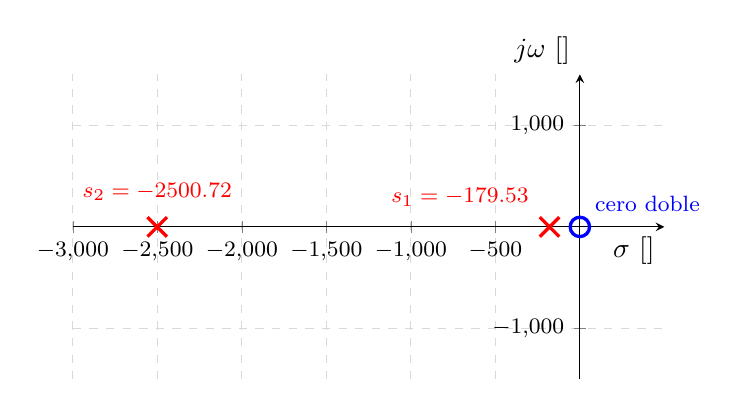
\begin{tikzpicture}
  \begin{axis}[
    width=0.75\textwidth, height=0.45\textwidth,
    axis lines=middle,
    xlabel={$\sigma$ [\unit{\radian\per\second}]},
    ylabel={$j\omega$ [\unit{\radian\per\second}]},
    xlabel style={at={(ticklabel* cs:1)}, anchor=north east},
    ylabel style={at={(ticklabel* cs:1)}, anchor=south east},
    xmin=-3000, xmax=500, ymin=-1500, ymax=1500,
    xtick={-3000,-2500,-2000,-1500,-1000,-500},
    ytick={-1000,1000},
    grid=both, grid style={gray!30, dashed},
    tick label style={font=\footnotesize},
    clip=false,
  ]
    \addplot[only marks, mark=x, mark size=5pt, very thick, red]
      coordinates {(-2500.72,0) (-179.53,0)};
    \addplot[only marks, mark=o, mark size=3.5pt, very thick, blue] coordinates {(0,0)};
    \node[above=6pt, red, font=\footnotesize] at (axis cs:-2500.72,0) {$s_2 = \num{-2500.72}$};
    \node[above left=4pt, red, font=\footnotesize] at (axis cs:-179.53,0) {$s_1 = \num{-179.53}$};
    \node[above right=2pt, blue, font=\footnotesize] at (axis cs:0,0) {cero doble};
  \end{axis}
\end{tikzpicture}
